\documentclass [12pt]{report}

\usepackage[magyar]{babel}
\usepackage[utf8]{inputenc}
\usepackage{t1enc}
\usepackage{graphicx}
\usepackage{multirow}
\usepackage{lscape}
\usepackage{lipsum}
\usepackage{geometry}
\usepackage{pdfpages}
\linespread{1.3}


\begin{document}
\includepdf[pages = {1}]{cucc.pdf}

\tableofcontents
\chapter{Bevezetés}
Ütemezési problémákkal az élet számos területén találkozhatunk, például hétköznapi feladatainkat is be kell osztanunk, az iskolában el kell osztani az órákat termekbe és a számítógép is ütemezi az elvégzendő folyamatait. Gyártórendszereknél jellemzően el kell osztani az adott erőforrásokat az azokon műveletet végző egységek között, így a gyártásütemezési feladatok az ütemezési problémák jelentős hányadát teszik ki. \\
A gyártásütemezés az iparra jellemző, a berendezéseken megadott idő alatt hajtanak végre műveleteket a termékeken. A végcél szempontjából az ütemezés célja lehet makespan minimalizálás vagy átviteli kapacitás (throughput) maximalizálás. Fontos a feladatokon elvégzett műveletek sorrendje, melyeknek a megadott módon kell egymást követniük.\\
Az irodalomban több lehetséges megoldó módszerről esik szó, gyártási probléma ütemezését elvégezték már többféle technika segítségével. A leggyakoribbak a MILP megoldó módszerek, melyek vegyes-egész lineáris programozáson alapulnak, de az S-gráf alapú megoldások is jellemzőek, valamint Petri-hálóval is oldottak már meg hasonló ütemezési feladatot.
Dolgozatomban egy gyártási probléma ütemezését választottam, amelyet költségfüggvénnyel kiterjesztett időzített automata használatával optimalizálok, és elemzem az eredményeket. Az időzített automata egy olyan automata, ahol órák segítségével modellezhetőek és korlátozhatóak az események.\\
Időzített automatával még nem járták körül bővebben a problémát, de érdemes vele foglalkozni, mert más problémaosztályok vizsgálata során hatékony módszernek bizonyult.\\
A feladat egy irodalmi példa, amelyben a meghatározott számú feladatot a gépek egy lépésben végzik el.
A feladat célja, hogy minél több feladatot elvégezzenek a gépek, és minél kevesebb legyen a kész termékek tárolási költsége.\\
A további megoldó módszerekkel elvégzett ütemezés eredményeiről szó esik a kapcsolódó irodalomban is, amelyeket fel tudunk használni arra, hogy az automatával elvégzett optimalizálás eredményeivel összehasonlítsuk őket. \\
Több modellt vizsgálunk meg, melyek eltérő korlátozási paraméterekkel rendelkeznek, így teszteljük az ütemezési folyamat lefutási idejét.

Dolgozatom második fejezetében az irodalmi háttérrel foglalkozom, a harmadik fejezetben részletezem a problémát, majd az időzített automatákról, a használt szoftverről és az LPTA alapú ütemezésről teszek említést. A negyedik fejezetben a teszteredményekről lesz szó, amelyeket korábbi megoldásokkal hasonlítok össze. A végén található az összefoglalás az ütemezés eredménye alapján, majd a dolgozat végére kerülnek a hivatkozások és a függelék. 


\chapter{Irodalmi áttekintés}
\section{Gyártási feladatok ütemezése}
Bármely gyártási ütemezési feladat rendelkezik közös vonásokkal, hasonló paraméterekkel, bármilyen módszert használunk a megoldáshoz. Közös bennük, hogy adottak a feladatok, a feladatokat elvégezni képes berendezések vagy eszközök, egy adott végrehajtási idő minden feladathoz, a cél pedig, hogy a kijelölt szempontok mellett megtaláljuk a lehető legjobb megoldást. Az egyes feladatok  végrehajtási ideje az az  időtartam, ami a munka elvégzéséhez szükséges, ez általában minden esetben egyedien meghatározott, tehát minden különböző feladatnak eltérő mennyiségű időre van szüksége. A feladatoknak lehet elvégzési határideje is, amit szintén figyelembe kell venni az ütemezés folyamán. Az irodalomban a feladatokat task megnevezéssel is használják, a munkát elvégző gépeket unit-ként, a termékeket pedig product-ként. \\\\
A problémákat különböző szempontok alapján lehet kategorizálni, az egyik csoportosítás alapján megkülönböztetünk sztochaikus és determinisztikus ütemezési feladatokat, ahol a sztochaikus típus azokat a problémákat jelöli, ahol a paraméterek futás közben kapnak értéket. A determinisztikus esetében az értékek előre be vannak állítva. \\
Egy másik csoportosítás szerint egy feladat a megadott paraméterek alapján lehet offline illetve online, ahol offline esetben a szükséges bemeneti adatok elérhetőek az ütemezés időpontjában, online esetben pedig a döntéseket meg kell hozni, mielőtt néhány paraméter értéke kiderülne. Az itt elemzett probléma az offline, determinisztikus feladatok körébe tartozik.\\
A különböző problémaesetek megoldhatóság szempontjából szintén kétféleképpen alakulhatnak. Ha az ütemezés nem elégít ki legalább egy korlátozást, akkor az nem megoldható (infeasible), minden egyéb esetben megoldható, tehát feasible. \\\\
A gyártási ütemezési feladatok egyik altípusa az egylépéses ütemezési probléma (single stage probléma), ahol a feladatokon egy tevékenységet kell végrehajtani, hogy azt befejezetté lehessen nyilvánítani. Az egylépéses problémák mellett vannak más gyakori típusok is, például a simple multiproduct, ahol a feladatot lineárisan több lépésben kell elvégezni, a general multiproduct, ami a simple multiproduct-hoz hasonló, de ki lehet hagyni lépéseket. A multipurpose (többcélú) problématípusban a lépéseknek nincs meghatározott sorrendje, tetszőlegesen hajthatóak végre. Megkülönböztethetjük a precedens típust, amely hasonló a többcélúhoz, de nem feltétlenül lineárisan hajtódnak végre a feladatok, és a general network típust, ahol a feladatokat az inputjaik és outputjaik alapján adják meg.\cite{Hegyhati2010}\\
  
A single stage problémáknak a megoldásához néhány paraméternek adottnak kell lennie, például a gépek számának, valamint annak, hogy ezek a gépek azonosak-e. Két gép akkor tekinthető azonosnak, ha ugyanazokat a munkákat képesek elvégezni ugyanannyi idő alatt. Szükség van továbbá a feladatok számára és típusára. \\\\
Az egylépéses ütemezési problémákat további alosztályokra lehet bontani, a gépek az alábbiakban felsorolt típusúak lehetnek.
\begin{itemize}
\item \textbf{1 - Single Machine:} Egy gép elérhető, amelyen minden feladatot végre lehet hajtani. A termékeknek (feladatoknak) különböző feldolgozási ideje van. 
\item \textbf{Pm - Identical paralell machines}(Azonos párhuzamos gépek): m számú azonos gép áll rendelkezésre, amelyeken bármelyik egylépéses feladat végrehajtható.
\item \textbf{Qm - Paralell machines with different speed} (Párhuzamos gépek különböző sebességgel): Hasonló az előző pontban említett típushoz, de minden gépnek meghatározott sebessége van.
\item \textbf{Rm - Unrelated machines in paralell}(Párhuzamos független gépek): Hasonló a Single stage típushoz, de a feladatok elvégzési ideje egy-egy gépen inputként meghatározott.  
\end{itemize}

\section{Megoldó módszerek}
Vannak olyan módszerek, amelyekkel már a legtöbb problémaosztály szempontjából foglalkoztak, így egylépéses gyártásütemezési feladatokkal is. Az alábbi néhány eljárás a legnépszerűbb megoldók közé tartozik.


\subsection{MILP modellek}
  A MILP modellek, tehát a vegyes-egész lineáris programozási modellek a legelterjedtebb megoldó módszerek közé tartoznak, és több altípusuk létezik.\\
  \emph{Time discretization based - Időfelosztásos módszerek:}\\
   Az időfelosztásos modellek előnye, hogy széles skálán mozog a megoldható problémák típusa.
  A módszer alapján időpontokat és időréseket különböztetünk meg, A MILP modellek időpontos megadást használnak gyakrabban.  \\
  Az időbeosztásos típusban a feladatokhoz bináris változókat rendelnek aszerint, hogy a feladat az adott időpontban elvégzésre kerül, vagy nem. Amikor a feladat abban az időpontban megvalósul, akkor 1 lesz a bináris változó értéke, ha nem, akkor 0. Így annyi bináris változóra lesz szükség, ahány időpontot meghatároztunk. Lehetőleg minél kisebb számú időpont felvételével kell megtalálni az optimális megoldást a modell bonyolultságának csökkentése érdekében.\\\\
  $x_{tij},$ ahol t időpont, i a feladat, j a berendezés\\ X értéke akkor 1, ha t időpillanatban j berendezés elvégzi i feladatot.\\\\
 \emph{Precedencia alapú modellek:}\\
  Szintén bináris változókat használ az ütemezéshez, de az időfelosztásossal ellentétben kettőt. \\
  $Y_{ij}$ értéke 1, ha i feladatot j berendezés elvégzi\\
  $X_{iji'}$ értéke 1, ha j berendezés elvégzi i és i' feladatokat úgy, hogy i-t előbb, mint i'-t.\\
  Az x változó segítségével megállapítható i és i' feladatok egymáshoz való viszonya a gyártási sorrendben. \\\\
 Két altípust különböztetnek meg az alapján, hogy az időpontokat az optimalizálás előtt meghatározzák, ezek a Fix időpontos időfelosztásos módszerek, vagy pedig csak a feladat közben kerül meghatározásra az időpontok száma. Utóbbiakat Variable time model-eknek hívják, és a lényegük, hogy minél kevesebb bináris változóra legyen szükség. A modellekben folyamatos változókat használnak, amik meghatározzák mindegyik időponthoz tartozó feladatokat \cite{Mendez2006}. 
 
 \subsection{S-gráf}
   Az első gráf alapú optimalizációra fejlesztett módszer a gyártásütemezés témakörében, amely nemcsak vizuálisan szemlélteti a folyamatot, de egyben egy matematikai modell is. Irányított gráfokból áll, amelynek a csomópontjai tevékenységek és az azokhoz vezető lépések, amelyeket az élek kötnek össze őket. Ezen kívül tartalmaznak ütemezési éleket, amelyek a meghozott ütemezési döntéseket modellezik.\\
   Létezik ütemezési döntések nélküli S-gráf is, ezt recept gráfnak hívják. \\
   A nyilak,  amelyek a csomópontokat kötik össze, a függőségeket reprezentálják.\cite{Smidla2010} \cite{Hegyhati2009}

\subsection{Petri háló és automaták}
A Petri hálót és az automatát is gyakran alkalmazzák diszkrét esemény rendszerű modellezéshez,? és hogy kötegelt feladatok elvégzéséhez is alkalmas legyen, ki kellett egészíteni  időzítéssel ezeket a módszereket?. Hatékonyak, mivel jól szemléltetik a modellt, könnyen szimulálható a felépítése és a vezérlés, és a megfelelő felépítés mellett elkerülhetőek a hibák. Bár több előnyük is van a korábban említett népszerű megoldó módszerekhez képest, összességégben hatékonyságuk még elmarad a MILP és S-gráf alapú megoldó módszerekétől, valamint optimalizálásra nem alkalmasak, csak a feladat modellezésére. \\
Az időzített Petri háló alapja, hogy az átviteli jel késleltetés (delay) alapján jön létre. Többen is foglalkoztak a témával, Ghaeli foglalkozott a kötegelt folyamatok ütemezésével ilyen módon, Soares pedig megpróbálta kiterjeszteni a modellt, és valós idejű ütemezést mutatott be kötegelt rendszerekre Petri háló segítségével. 

\section{Az ütemezés ábrázolása}
Az ütemezési feladatok megoldását Gantt diagramon ábrázolják. A példa három berendezést jelöl az y tengelyen (E1, E2, E3), az x tengelyen pedig az eltelt idő látható percben megadva. A diagram azt mutatja be, hogy egyes berendezések mikor végezték el a feladatokat, amelyek A-val, B-vel és C-vel vannak jelölve. A Gantt diagramról leolvasható, hogy melyik munka mikor kezdődött, és mikor fejeződött be, ebből adódóan pedig megállapítható, hogy milyen hosszú ideig tartott. \cite{Ghaeli2005}
\begin{figure}[h]
\begin{center}
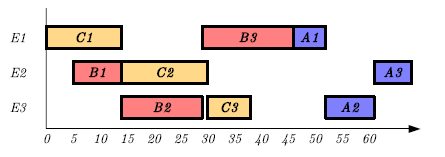
\includegraphics{gantt}\\
\caption{Példa egylépéses ütemezési feladat ábrázolására Gantt diagramon}
\end{center}
\end{figure}

 

\chapter{Időzített automaták}

\section{Időzített automaták}
 Egy automata eseményekből és állapotokból áll, az időzített automata pedig kiegészül órákkal, amelyek mérik a globális időt, vagy egy konkrét automata idejét. \\
 Az időzített automata a determinisztikus automaták csoportjába tartozik, ahol a determinisztikus automatákat az alábbi képlettel adják meg.\cite{Subbiah2009}
 \begin{center}
 M = (K, $\Sigma$, $\delta$, s, F)
 \end{center}
 ahol\\
 \indent \textbf{K} az állapotok halmaza\\
 \indent $\mathbf{\Sigma}$ az események véges halmaza\\
 \indent \textbf{$\delta$}: K x $\Sigma$ $\rightarrow$ K részleges átmeneti függvény\\
 \indent \textbf{s} a kezdőállapot\\
 \indent \textbf{F} az elfogadó állapotok \\\\
 
 Egy időzítés nélküli determinisztikus automata az \ref{tab:det} ábrán látható módon épül fel.\\
 \begin{figure}
 \begin{center}
 \label{tab:det}
 \includegraphics[width=12cm]{det}
  \caption{Determinisztikus automata}
 \end{center}
 \end{figure}
 
 Az automata két állapotból áll, valamit \emph{a, b} eseményekből, az élek mutatják, hogy melyik állapotból milyen események hatására melyik állapotba kerülhet az automata. Ez alapján megállapíthatunk olyan szavakat, amelyek végig tudnak futni, és vannak olyanok is, amelyek nem.\\\\
 1. példa - szó, ami lett tud futni\\
 aaba - Az első állapotból átmegy a másodikba az \emph{a} eseménnyel, ugyanígy a harmadikba, majd a harmadik állapotból \emph{b} esemény hatására ugyanebben az állapotban marad. Végül \emph{a}-val eljut a végső elfogadó állapotba. \\
 2. példa - nem megfelelő szó\\
 aba - Eljut a második állapotba \emph{a} esemény hatására, de a második állapotból csak egy újabb \emph{a} eseménnyel tudna átkerülni a harmadik állapotba, viszont a szó \emph{b}-t tartalmaz, így nincs olyan él, amelyen tovább tudna haladni.\\
 

 
 
Az időzített automaták kiegészülnek órákkal, amelyek stopperóraként működnek, tehát a globálisan deklarált óra az automata teljes lefutási idejét méri.\\
	Egy átmenet csak akkor történhet meg, ha az időzítési feltétel teljesült, az átmenet után az órák akár vissza is állíthatók. Ezekben az esetekben általában a feladatokat és a berendezéseket külön modellezik, és paralell composition használatával kapcsolják őket össze. A külön modellezés eredményeképpen az elkészült modell nagy lesz, és bonyolult bemutatni, mégis az eredmények megalapozottak. \\
Az időzített automata képlete:\\
\begin{center}
$(K, \Sigma, C, Tra, Inv, s)$\\
\end{center}
ahol\\
\indent \textbf{K} az állapotok halmaza\\
\indent $\mathbf{\Sigma}$ az események halmaza\\
\indent \textbf{C} az órák halmaza\\
\indent \textbf{Tra} K x $\phi$(C) x $ \Sigma $ x C x K időzített transitions\\
\indent \textbf{Inv} K $
\rightarrow  \phi$(C) state invariants -\\
\indent \textbf{s} a kezdőállapot \\
Az időzítést egy egyszerű szó levezetésével tudjuk bemutatni, ahol az események meghatározott időben történnek.\\
Példának vesszük az (a,1) (b,3) (a,4) (b,6) (b,10) időzített szót.\\
A fenti felírás azt mutatja, hogy melyik időpillanatban történik az esemény, amiből kiszámíthatjuk, hogy a betűk mennyi késleltetéssel követik egymást. 
\begin{center}
d1$\rightarrow$ \textbf{a} $\rightarrow$d2$\rightarrow$ \textbf{b} $\rightarrow$d1$\rightarrow$ \textbf{a} $\rightarrow$d2$\rightarrow$ \textbf{b} $\rightarrow$b4$\rightarrow$ \textbf{b}
\end{center}
ahol \emph{d} a késleltetést (delay-t) mutatja.\\
Az első \emph{a} 1 delay eltelte után kezdődhet el, és mivel \emph{b} 3 delay után következik, \emph{a}-t követően 2 delay-t kell várnia, a következő betűk pedig ennek alapján ugyanezt a szabályt követik.\\
Az időzített automatát a label ábrán mutatott példán láthatjuk. Minden átmenet három részből áll, a korlátozásból, az eseményből, és a visszaállított értékből (guard, event, reset). \\
Az események \emph{msg} és \emph{reset}, c1-el az órát jelölik, az állapotok 0 és 3 között sorszámozottak. A 0 és 1 állapot között nincs korlátozás, ezért átmehet az 1-es állapotba \emph{msg} esemény hatására, az órát visszaállítja. \cite{Behrmann2005} \cite{Panek2008}\\

\section{UPPAAL Cora}
A választott irodalmi példa időzített automatákkal való ütemezését az UPPAAL Cora nevű szoftver segítségével modelleztük. A szoftver alkalmas az automaták modellezésére, ütemezésére és optimalizálására meghatározott paraméterek alapján. \\
Az UPPAAL segítségével sablonokat (template-eket) hozhatunk létre, ahol minden egyes template egy különböző automata modellezésére szolgál. A sablon állapotokat és éleket tartalmaz, ahol az élek az állapotátmenetet szimbolizálják. \\
Az állapotokhoz megadhatunk nevet, illetve valamilyen korlátozást, ezen kívül beállíthatjuk az állapotát, ami initial, urgent vagy committed lehet. Az initial az automata kezdőállapotaként jelöli meg a kijelölt státuszt, a committed még inkább korlátozó, mint az urgent, tehát nem késleltetheti a következő átmenetet. Ugyanitt beállítható az is, ha az adott állapotban növekszik a költség valamely egyéb korlátozásból adódó várakozás miatt. Ekkor az állapot beállításaiban az Invariant pontban adható meg az idő előrehaladásával számított költség mértéke. \\
Az irányított élek mutatják, hogy melyik állapotból melyikbe van lehetőség átkerülni, ezen kívül pedig egyéb beállítások is megadhatóak. Minden élre megadható  Select, Guard, Sync és Update információ. A Select-ben nemdeterminisztikus választásra van lehetőség, a Guard korlátozást állít be, aminek teljesülnie kell, hogy a feladat a következő állapotba kerüljön. A Sync lehetőséggel különböző automaták állapotátmeneteit lehet összehangolni, ehhez csatorna létrehozására van szükség. Az Update segítségével frissíthetőek a változók értékei és az órák.\\
Az automata template-ek az Editor menüpont alatt helyezkednek el, és itt található még a Declarations menüpont is. 
\begin{figure}
\begin{center}
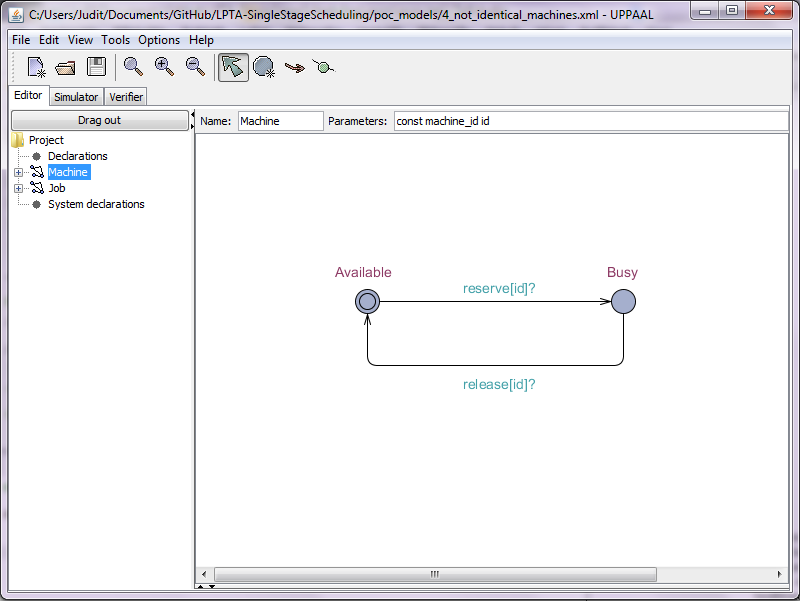
\includegraphics[width=10cm]{uppaal2}
 \caption{Az UPPAAL Cora Editor ablaka}
\end{center}
\end{figure}
A  Declarations pontban az egész rendszerre vonatkozó változókat és értékeket lehet megadni, valamint függvényeket létrehozni. Az értékeket egészként kell meghatározni, mert a szoftver nem számol lebegőpontos alakban. Definiálhatunk órákat (clock), illetve csatornákat (chan), ezek az automaták közötti szinkronizálást segítik elő.\\
Minden template-hez definiálhatunk lokális változókat és paramétereket, ahol a paraméterek segítségével például meg tudjuk különböztetni a példányokat, ha a modell példányosítva van. Ekkor hozzárendelünk egy ID-t, amely sorszámot ad az automatáknak. A lokális változók között gyakran definiálunk órát, ha például egy elvégzendő feladatról van szó, külön mérhessük a munkaidejét, amit ilyenkor a modell elején le is kell nullázni.\\ 
Az Editor lapon található még a System Declarations pont, ami az automaták konkrét példányosítását végzi.\\
Az Editor mellett két fontos menüpont található. Ha nem vétettünk szintaktikai hibát, a szimulátor betölti a létrehozott automaták összes példányát, mellette pedig megjeleníti a változókat, amelyek először a kiinduló állapotban vannak, ahogy az automaták is. Itt lehetőség van egy megoldást lefuttatni, ekkor szinte biztos, hogy nem az optimális eredményt kapjuk. A lépéseket saját magunk is kiválaszthatjuk, a végeredményt pedig mindkét esetben vissza lehet játszani, vagy elmenteni egy külön fájlba.  \\
A szimulátor közben bemutatja, hogyan változtak az értékek, hogy az automaták melyik állapotukban vannak, valamint egy másik ábrán szekvencia diagramon láthatjuk a szinkronizáció lépéseit, és az automaták állapotátmenetét.\\
\begin{figure}[htpb]
\begin{center}
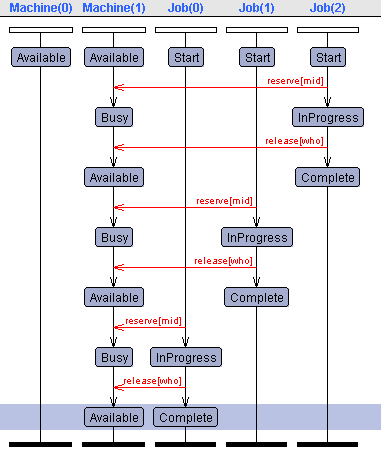
\includegraphics[height=10cm]{szekvencia}
\caption{A folyamat szekvenciadagramja}
\end{center}
\end{figure}
A 4.2 ábrán látható egy példa egy minta szekvenciadiagramot árázol, ahol két gépen három feladat kerül felosztásra, és bemutatja a szinkronizációs csatornák működését az egyik megoldásban.\\
A harmadik menüpont a Verifier, itt a Query-ben meg lehet adni lekérdezéseket, amelyet az UPPAAL lefuttat, majd kiírja az eredményt amely két fajta lehet. Ha a beírt korlát alapján talált megoldást, akkor megkapjuk a \emph{Property is satisfied} üzenetet zölddel kiírva a Status pont alatt.  Az UPPAAL a TCTL logika egyszerűbb formáját használja a query nyelvében.\\
 Az Overview-nál is megjelenik a megadott Query, mellette pedig egy zöld jel. Ellenkező esetben a \emph{Property is not satisfied} üzenetet kapjuk, az Overview pedig piros jelet tesz a Query-ben megadott korlát mellé.    \\
A főmenüben leginkább az általános lehetőségeket találjuk, a Tools és az Options pontokban találhatóak egyéb beállítások az automaták ütemezésével kapcsolatban. Leellenőrizhető a Declarations és a template-ek definiálása során megadott adatok és korlátozások szintaktikai helyessége, az Options pedig az ütemezési beállításokat tartalmazza. \\
Átállítható például, hogy ütemezés során mélységi, szélességi vagy egyéb keresést alkalmazzon, valamint hasznos funkció, hogy ha a Diagnostic Trace értékét some-ra állítjuk, akkor abban az esetben, ha a Query-ben definiált lekérdezés teljesül, a megoldást be tudja tölteni a szimulátorba. A szimulátorban grafikusan, diagramon és változónként is elemezhető az eredmény. \\
Az UPPAAL Cora-hoz Java Runtime Enviroment szükséges, mivel a felhasználói interfész Java nyelven van implementálva.

\chapter{Problémadefiníció}
A probléma egy egylépéses szakaszos eljárás ütemezéséhez kapcsolódik, ahol minden termék egy termelési lépés alatt készül el, ezeket a hívjuk munkáknak. A munkákat bármelyik gép (unit) elvégezheti, de egy munka csak egy géphez rendelhető hozzá. Ugyanígy egy gép egyszerre csak egy feladaton dolgozhat, és ha már egy munkát elkezdett, azt egy másik nem előzheti meg. \\
Az egylépéses ütemezési problémákat általában táblázat segítségével adják meg, ahol a sorokban tüntetik fel a munkákat, az oszlopokban pedig a rendelkezésre álló berendezéseket, a táblázatbeli metszéspontjaik ábrázolják az egyes munkák megfelelő berendezéseken való elvégzésének munkaidejét. Kopanos részletesen foglalkozott egylépéses ütemezéssel. \cite{Kopanos2009}\\
Adott a munkák és a gépek száma, valamint a gépeknek van egy meghatározott üzembe állási ideje, ez mindegyik berendezés egyedi tulajdonsága. Két munka elvégzése között felszámolunk átállási időt, amíg a gép testre szabja saját beállításait a következő feladathoz. A gyakorlatban ez tisztítást, újra beállítást és egyéb karbantartást jelent. Az átállási időt kétféleképpen lehet megadni, az egyik típus a szekvenciafüggő, amikor a feladatok sorrendje határozza meg az értéket. Mennyiségét az szabja meg, hogy az előző és az utána következő munka között mennyi időre van szüksége a berendezésnek. A másik megadási mód a szekvenciafüggetlen típus, amikor csak a berendezéstől függ az átállási idő. Mindkét modellt be lehet állítani úgy, hogy minkét típus függjön a géptől és a feladattól is. \\
A munkákat minden gép különböző idő alatt tudja elvégezni, de olyan eset is lehet, amikor egy gép nem tudja elvégezni az adott munkát. Minden feladat rendelkezik határidővel, amit nem léphet át, miközben várakoznia kell, ha a határidő előtt elkészül. Az ütemezés célja, hogy minimalizáljuk a várakozás költségeit, emellett viszont előfordulhat, hogy a megoldás nem elégít ki a korlátozásokat, így infeasble lesz. Ha van feasible megoldás, szeretnénk lehetőleg az összes munkát elvégezni határidőre, valamint a modellt kiegészíteni korlátozásokkal úgy, hogy minél kevesebb idő alatt elvégezze az ütemezést, és minél optimálisabb eredményt adjon.  \\
A feladatban munkákat és gépeket különböztetünk meg, amelyeket később P-vel és U-val jelölünk, a product és unit szakirodalomban használt megnevezések után. \cite{Behrmann2001}
 
  

\chapter{Egylépéses feladat LPTA modellje}
    Az LPTA modell két template-ből, a rendszer deklarációkból és a változó deklarációkból áll. A template-ek egy-egy automatát írnak le, valamint saját változókkal is rendelkeznek, ezeket később részletesen be fogjuk mutatni. Ebben a példában a két sablon a gépeket és a feladatokat modellezi.\\
    A következő fejezetekben részletesen bemutatjuk a két template-et, a lekérdezéseket és a definiált paramétereket.
    \section{Modell 1}
    \subsection{Deklaráció}
     A template-ek meghatározásához a deklarációban adtuk meg a szükséges paramétereket, illetve függvényeket, amelyek szükségesek az automaták ütemezésének futtatásához. Meghatároztuk a gépek és a feladatok számát, ami az irodalmi példa szerint négy gépet és huszonöt feladatot jelent, majd ezeknek kiosztottunk egy saját azonosítót. Szintén a globális deklarációban definiáltuk a munkaidőket gépek szerint, hiszen minden gép más-más idő alatt tud elvégezni egy feladatot. Ugyanígy megadtuk a határidőket, átállási időt, a beállási időt és a csatornákat is.\\
     A modell három csatorna tömböt tartalmaz, amelyek a \emph{foglal, elenged} és \emph{kezdődik} elnevezésűeket, ezek mindegyike annak a gépnek a sorszámát tárolja el paraméterben, amelyiken a feladat végrehajtódik.\\ 
      Deklaráltuk a globális órát, amely az ütemezés kezdetétől méri az összes időt, amíg az utolsó lépést el nem végzi, ezen kívül a \emph{feladat} és a \emph{gép} template rendelkezik külön órával. A feladat sablon a munkaidővel és a határidővel hangolja össze a saját óráját, a gép pedig a saját beállási idejét méri vele. 
      A deklaráció szintaktikája három fő elemből épülhet fel.\\
       A template típusú elemek, melyek közé tartoznak a csatornák, ezeket \emph{chan}-ként hozhatjuk létre, valamint ide tartoznak az int típusú változók is, amelyek az ütemezés során többször is értéket kaphatnak. A csatornákat is lehet tömbként létrehozni, az általam létrehozott modellekben annyi csatornát hoztam létre, ahány gép áll rendelkezésre, így a catorna létrehozásakor paraméterként a gépszámot tartalmazó konstans integer értéket kapta meg. \\
      A második nagyobb csoport a konstansoké, ezeket a futtatás előtt deklaráljuk, értéküket nem változtatják, manuálisan kell őket beállítani. Ezeknek mindenképpen integer értéket kell adni, létrehozásuk a \emph{const int név} formában lehetséges, ahol a const jelzi, hogy statikus értékről van szó, a \emph{név} helyére kerül a konstans neve.\\
       A modelljeim létrehozásakor a munkaidők, a munkaszám, a gépszám, az átállási idők, a beállási idők és a határidők is konstansként kerültek létrehozásra, hiszen ezek az értékek előre megadottak, és nem változtathatók meg.\\
       A munkaidő és az átállási idő értékek kétdimenziós tömbben vannak tárolva, ahol a munkaidők esetében az egyik érték a munkaszám, a másik a gépszám, mivel minden gépen minden feladat más munkaidővel rendelkezik. A munkaszámokat nem a \emph{munkaszám} változóval adtam meg, mivel ha változtatni próbálnánk a munkaszám értékét (amire a tesztelés során szükség lesz), a munkaidő szintaxis hibát jelezne amiatt, hogy az egyik paraméter megváltozott, a deklarált értéksorok száma viszont nem. Azzal, hogy konstans értékkel szerepel a munkaszám, az érték megváltoztatható, de a munkaidő értékek sem lesznek hibásak. \\
       Az átállási időt szintén kétdimenziós tömbként hoztam létre, ahol a korábban említett probléma elkerülése okán konstans számokként határoztam meg a munkaszám értékeket. 
      A korlátos integer változók a harmadik csoport. Korlátok, invariánsok, feladatok is tartalmazhatnak korlátos integer változókat, ezek a verifikáció során ellenőrzésre kerülnek, és ha megsértik a korlát értékeket, érvénytelen állapotot eredményeznek, ami eldobásra kerül futtatáskor. Ezeket a változókat az \emph{int[min,max] név} formában lehet létrehozni, ahol a min és a max értékek jelentik a felső és az alsó korlátokat. Ha a korlátokat elhagyjuk, az alapértelmezett értéktartomány -32768-tól 32768-ig tart.\\
      A fent említett elemeken kívül léteznek még különböző típusok, ezek közül a C nyelvhez hasonló typedef konstruktort használtam, amellyel egyéni vagy alap típusokat lehet definiálni értékek számára. A deklarációban a munkák, illetve a gépek sorszámainak tárolására hoztam létre egy \emph{typedef int} típusú változót, amely egyben korlátos is, mivel egy 0-tól a megadott munkaszámig tartó intervallummal került paraméterezésre.
      \\
      
    \subsection{Template-ek}
    A modellben két különböző template-tel dolgozunk, ezek a Gép és Feladatok elnevezésű sémák. Mivel az ütemezést több különböző változatra bontottuk, itt az első modell kerül bemutatásra, amely nem tartalmaz korlátozásokat az ütemezési folyamat gyorsításának szempontjából.\\
    A template-ek létrehozásakor az éleknél és az állapotnál különböző beállításokra volt szükség, ahol a modell a deklarációban létrehozott változókat és értékeket felhasználja.
    Az élekhez tartozó szerkesztési ablakban van lehetőség arra, hogy ezekkel beállítsuk a szükséges korlátozásokat, szinkronizációt, valamint frissítsünk vagy kiválasszunk értékeket.\\
    Az élek szerkesztési ablakában a \emph{Select, Guard, Syncronisation} és \emph{Update} pontok találhatóak meg. A Select egy \emph{név:típus} formájú kifejezést vár, ahol a név a változó neve lesz, a típus pedig egy már létrehozott típusdefiníciós változó. Ezzel egy változóba menthetjük el például a feladat által befoglalt gép sorszámát, mint ahogy ez a Feladat template paraméterezése során is megtörtént. \\
    A Guard egy olyan korlátozási kifejezés, amely boolean értéket ad vissza, emiatt csak integer, konstans vagy óra értékre lehet alkalmazni. Órákat csak integerekkel lehet összehasonlítani. Az első modellben automatájában a legtöbb élen vannak korlátozások, amelyek teljesülése esetén kerülhet az automata a következő állapotba. A szintaxis nyelve hasonló a C programozási nyelvhez, operátorokkal tudjuk kifejezni a feltételt. A Feladat template-ben az első élen a munkaidő nem lehet 100000, amelyet != operátorral állítunk be.\\
    A bináris csatornák használatakor a két template közti szinkronizációt a létrehozott csatorna címkézésével lehet beállítani. Például a \emph{kezdődik} csatorna úgy hangolja össze a két template-et, hogy a megfelelő él szerkesztési ablakában a szinkronizációs beállításoknál megadjuk a csatorna nevét, a hozzá tartozó paramétert, ez pedig eltárolja a gép sorszámát. Az összehangolást a ? és !  operátorok végzik el, tehát az egyik template-ben létrehozott \emph{kezdődik[id]!} csatorna a másik template \emph{kezdődik[id]?} csatornájával szinkronizál.\\
    Az Update lehetőségnél vesszővel elválasztva frissítési értékeket adhatunk változóknak, konstansoknak vagy óráknak. Az update pont az egyetlen az említettek közül, amelynek side-effect hatása lehet, mivel változtathat a korábbi értékeken. Az első modellben frissítéssel adunk értéket például akkor, amikor az aktuális és az előző munkát akarjuk frissíteni. Az aktuális értéket az automata első élén állítjuk be, majd a feladat elvégzése után átállítjuk, mivel elvégzésre került, és az azonos gépen elvégzendő következő feladat átállási idejénél ennek a feladatnak és az elvégzendő kiválasztott feladatnak az átállási idejét kell figyelembe venni.\\
    A későbbi modellekben használjuk a committed állapotot, amely nem engedi meg, hogy a következő átmenet késleltetve történjen meg.\\
    A template-ek számára lokális paramétereket is deklarálhatunk, ezeket a template-ek feletti \emph{paraméterek} lehetőségnél lehet létrehozni, és csak az adott automata számára lesznek elérhetőek. \\
    
    \subsubsection*{Gép template}
    Az Gép elnevezésű template azt a minta gépet modellezi, amelyen a feladatokat el kell végezni. Három fő állapota van, ezek a kikapcsolt, bekapcsolt és a dolgozik. Kikapcsolt állapotból indul, és akkor kerül át bekapcsoltba, ha letelt az adott gépnek szükséges beállási idő, ezután kezdhet el dolgozni.  Ha a berendezés már bekapcsolt állapotban van, egy feladat befoglalhatja, ezt a \emph{foglal} csatorna szinkronizálja, annak a gépnek az automatája lép át a következő állapotba. Mielőtt \emph{Dolgozik} állapotba jutna, meg kell vizsgálnia, hogy az azon a gépen ez lesz-e az első elvégzett munka, mivel két munka elvégzése között átállási időt számol fel. Ha előtte nem dolgozott, akkor átállási idő nincs, a berendezés átvált \emph{Dolgozik} állapotba a \emph{kezdődik} csatorna segítségébel. Ellenben ha egy másik munka már megelőzte a jelenlegi munkát, az eltárolt aktuális és előző feladat azonosítója alapján ki kell várnia a hozzájuk tartozó átállási időt, és csak azután kezdheti meg a munkát. \\
    A \emph{foglal} csatorna közben szinkronizálja a gépet a feladat modelljével, a munkaidő letelte után pedig mindkét automata az \emph{elenged} csatorna segítségével jut a következő állapotba, ami a gép esetében a bekapcsolt állapot, ekkor vár az újabb feladat érkezéséig. Itt váltja át az előző munka azonosítóját, hiszen az elvégzett munka a következő lefutás során már az előző munkának fog számítani. 
    \begin{figure}[htpb]
    \begin{center}
   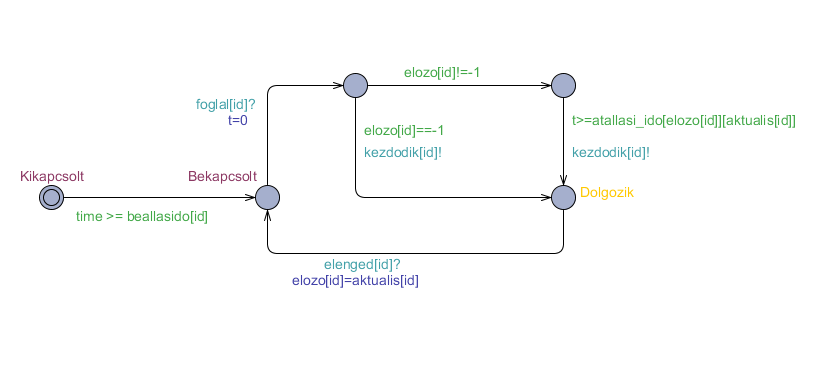
\includegraphics[width=12cm]{gep}\\
    \caption{A gép automatájának modellje}
    \end{center}
    \end{figure}\\
    \subsubsection*{Feladat template}
    A másik template a \emph{Feladatok}at mutatja be.\\
    Ez a modell öt állapotot tartalmaz, ebben az esetben a feladat a \emph{Start} stádiumból indul, ekkor a munka arra vár, hogy befoglalhasson egy gépet. Amikor ez megtörténik, átlép a \emph{Gép befoglalásra vár} elnevezésű állapotba, előtte viszont a \emph{foglal} csatorna segítségével szinkronizálja a saját státuszát a befoglalt gép státuszával, valamint elmenti, hogy aktuálisan hányas azonosító számmal rendelkező gépen kerül elvégzésre, ami fontos a munkaidő szempontjából, hiszem a saját magához tartozó munkaidőt kell felszámolni a gépen, és a gépnek is tudnia kell, hogy a korábban említett beállási időt meg tudja állapítani. Ezen kívül lekorlátozzuk, hogy ne olyan gépet foglaljon le, amely nem tudja a munkát végrehajtani, ezt a munkaidők megadásánál kiugróan magas számmal különböztettük meg, egységesen 100000-rel. \\
    A \emph{Gép befoglalásra vár} állapotban arra vár, hogy a befoglalt gépet beállítsák, ekkor kezdődhet el a feladat elvégzése. Minden feladathoz tartozik egy lokális óra, amelyen a munkaidejét méri, ezt a feladat kezdete előtt lenullázzuk, hogy a munka elkezdésétől számítsa annak munkaidejét. A gép beállítása után addig tartózkodik a \emph{Dolgozik} állapotban, míg a munkaideje le nem telik, ekkor újra szinkronizálja a saját és a gép státuszát, hogy a gép felszabaduljon, a feladat pedig átkerülhessen \emph{kész} állapotba. \\
    A \emph{kész} állapot azonban még nem azt jelenti, hogy a munka elkészült, hiszen a cél az, hogy pontosan a határidő leteltekor legyen leszállítva, ezért minél hamarabb készült el, annál többet kell várakoznia. Ebben a státuszban számoljuk fel a várakozás költségeit, amelyek az idő függvényében lineárisan növekednek. \\
    Amikor elérkezik a meghatározott határidő, a munka leszállításra kerül, ez a végső \emph{leszállítva} állapot.  
    \begin{figure}[htpb]
        \begin{center}
        \label{tab:gepautomat}
       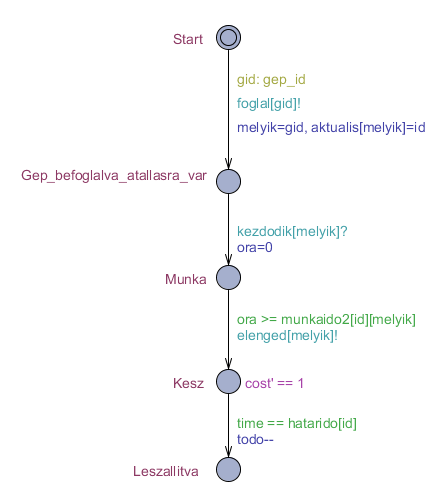
\includegraphics[height=8cm]{Feladat}\\
        \caption{A gép automatájának modellje}
        \end{center}
        \end{figure}
    \\    
   
    \subsection{Lekérdezések}
    A lekérdezések segítségével adjuk meg, hogy milyen kitételt szeretnénk leellenőriztetni az ütemezés során, melyre pozitív vagy negatív válasz érkezik. A jelenlegi modellben a feltétel, amit megvizsgáltattunk az volt, hogy létezik-e olyan megoldási lehetőség, ahol minden feladat kész lesz határidőre.\\
    Hogy a lekérdezés szerkezetét leegyszerűsítsük, bevezettünk a deklarációban egy változót, amelynek értéke minden esetben megegyezik a munkaszámmal. Amikor a feladat a \emph{kész} állapotból \emph{leszállítva} állapotba kerül, ezt az értéket mindig egyel csökkentjük, így optimális esetben, tehát ha minden feladat elkészül, nulla értéket vesz fel. Így a lekérdezés az alábbi módon kerül megadásra.
    \begin{center}
	\emph{E<> todo==0}
    \end{center}
    Ez a forma egyszerűbben megadható, és kiváltja a plusz változó nélküli hosszú megadást, ahol egyesével kellene ellenőrizni, hogy az adott feladat elkészült-e. \\
    Az ábrán a gép automatájának modellje látható \ref{tab:gepautomat}.
    
\section{Továbbfejlesztett modellek}
\subsection{Modell 2}
A modell második változatában a \emph{gép} template harmadik állapota az előzőhöz képest \emph{committed} minősítést kapott, tehát ebben az állapotban nem történhet késleltetés, mindenképpen tovább kell haladnia a következő állapotba, ami a \emph{dolgozik} állapot, de előtte megvizsgálja, hogy volt-e előző feladat. Ha volt, akkor a beállási időt kell kivárnia, ezután mehet át a \emph{dolgozik} státuszba.\\
\begin{figure}[htpb]
\begin{center}
\includegraphics[height=6 cm]{modell2}
\caption{A modell 2}
\end{center}
\end{figure}
A másik módosítás a \emph{feladat} template \emph{Start} állapotában történt. Itt hozzáadtunk egy korlátozást, amely megakadályozza, hogy ha kevesebb idő áll rendelkezésre a határidőig, mint az aktuális feladat munkaideje, akkor sem maradhat abban az állapotban. Ezzel olyan lefutási lehetőségeket zárunk ki, amelyek nem vezetnének megoldáshoz, viszont növelik a modell méretét, ezzel pedig megnövekszik az ütemezés futtatásának ideje.
\begin{figure}[htpb]
\begin{center}
\includegraphics[height=10 cm]{modell2_f}
\caption{A modell 2 Feladatok template-je}
\end{center}
\end{figure}
\subsection{Modell 3}
A \emph{gép} sablon \emph{committed} és \emph{dolgozik} állapota között van egy átmeneti állapot, ahova akkor jut a gép, ha már nem az első feladaton dolgozik, ezután vizsgálja meg, hogy milyen hosszú beállási időre van szükség az előző feladatot figyelembe véve. A Modell 3-ban korlátozzuk azt az időt, amíg a gép ebben az állapotban tartózkodhat, ami ezután nem lehet több, mint az előző és az aktuális munka alapján megállapított átállási idő. \\
 \begin{figure}[htpb]
    \begin{center}
   \includegraphics[width=15cm]{modell3}\\
    \caption{A Modell 3}
    \end{center}
    \end{figure}\\
Továbbá a \emph{dolgozik} állapotban sem tartózkodhat tovább, mint a feladathoz szükséges munkaidő, ezzel pedig megelőzhető, hogy a gép \emph{dolgozik} állapotban maradjon, ha a feladat a \emph{munka} státuszból nem tud átmenni a \emph{kész} állapotba, így nem is engedné el a gépen, amit korábban befoglalt. Ennek segítségével a berendezés csak addig lehet \emph{dolgozik} állapotban, amíg le nem telik a tevékenységhez szükséges idő, utána mindenképp fel kell szabadítani a gépet.\\
A korlátozás segítségével nem maradhat elfoglalt a gép egy olyan munkával, ami meghatározott időn belül nem tud befejeződni. \\
A \emph{feladat} template-be még három korlátozás került, a \emph{gép befoglalásra vár} státusz után akkor foglalhat be gépet, ha több idő áll rendelkezésre, mint amennyivel nem tudna befejeződni a saját határidejéig. \emph{Munka} állapotól \emph{kész állapotba} akkor válthat át, ha nem haladta meg a határidőt, ugyanígy akkor léphet tovább a \emph{kész} állapotból, ha a határidőig még van idő.\\
A modell 3-ban a \emph{gép} template átállási idővel kapcsolatos korlátozása változott, itt megengedjük az egyenlőség mellett azt is, hogy az óra magasabb értéket mutasson. A \emph{feladat} sablonban hasonló módon a \emph{munká}ból a \emph{kész} állapotba akkor is átválthat, ha a saját órája értéke nem feltétlenül egyenlő a feladat munkaidejével, de nagyobb is lehet.
\begin{figure}[htpb]
    \begin{center}
   \includegraphics[width=9cm]{modell3_f}\\
    \caption{Modell 3 Feladat template}
    \end{center}
    \end{figure}
\subsection{Modell 4}
A negyedik modell egy kisebb változtatást tartalmaz a harmadik modellhez képest, méghozzá ahol a modell átválthat \emph{Dolgozik} állapotba. Ebben a verzióban legalább az átállási időnek el kell telnie, hogy a következő státuszba jusson, de nem szükséges pont az átállási idő leteltekor ennek megtörténnie, később is bekövetkezhet.\\
Ezen kívül a Modell 4 működése megegyezik a Modell 3-mal.
 \begin{figure}[htpb]
    \begin{center}
   \includegraphics[width=12cm]{modell4}\\
    \caption{Modell 4 Gép template}
    \end{center}
    \end{figure}\\ 
 
\subsection{Modell 5}
Az ötödik modell egy template-ből áll, ez pedig a feladatok automatája. Itt egy modellben kezeljük a gépekre vonatkozó adatokat, ez az automata négy állapotból áll, amelyek a \emph{Start, Elkezdve, Kész} és \emph{Leszállítva}. Az állapotok a modell 3-hoz hasonlóan korlátozottak.\\
\begin{figure}[htpb]
\begin{center}
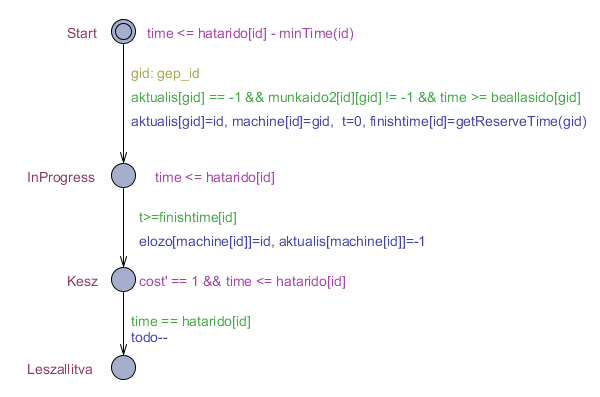
\includegraphics[height=6.5 cm]{modell_5}
\caption{A modell 5}
\end{center}
\end{figure}
 A \emph{Start} státuszból akkor kerül át \emph{InProgress} állapotba, ha megfelel néhány korlátozásnak. A munkaidő értéke nem lehet -1, ez azt jelenti, hogy azon a gépen nem lehet elvégezni az adott feladatot. A beállási időnek el kell telnie, ezért az óra állása nem lehet kisebb, mint ez az érték. Ha ezek a feltételek teljesülnek, elmentjük a munka azonosítóját és a gép azonosítóját, lenullázzuk az órát. A \emph{getReserveTime} függvényt a deklaráció tartalmazza, ezzel a függvénnyel megvizsgáljuk, hogy azon a gépen az aktuális feladat lesz-e az első, és ha nem, akkor a munkaidőt adja vissza, különben nullát. Ezt a számot a \emph{finishtime} nevű változóban tároljuk el.\\
 A következő két állapot közti átmenet akkor történhet meg, ha letelt a finishtime-ban megállapított idő, ezután pedig a modell visszaállítja az \emph{aktuális} változó értékét, az \emph{előző}t pedig frissíti az abban a pillanatban aktuális feladat azonosítójára, mivel a következő lefutás során ez már az előző munkának fog megfelelni. \\
 A \emph{kész} és \emph{leszállítva} státuszok közti átmenet a korábbi modellekhez hasonlóan alakul, az óra meg kell, hogy egyezzen a határidővel, a még elvégzésre váró feladatok számát pedig csökkentjük.

\subsection{Modell 6}
A következő modell elkészítése során hasonló megközelítést alkalmaztam, mint a Modell 5 esetén, viszont ebben az esetben a \emph{Gép}eket ábrázoltam automatával, a feladatok pedig tömbös szerkezet segítségével kerültek bele a modellbe.\\
A \emph{Gép} automata felépítése hasonlít a korábbi Gép automatákéra, ugyanúgy \emph{Kikapcsolt, Bekapcsolt} és \emph{Dolgozik} állapotokból áll, és az átállási időt is kezeli. Mivel nincs a feladatoknak külön template-je, nincs szükség szinkronizálásra. A feladatok sorszámát az \emph{id} változó tárolja.\\
\begin{figure}[htpb]
\begin{center}
\includegraphics[height=5 cm]{modell6}
\caption{Modell 6}
\end{center}
\end{figure}
Bevezetésre került egy \emph{állapot} tömb, amely a feladatok aktuális állapotát tartalmazza az indexek alapján. Három értéket vehet fel (0, 1, 2) aszerint, hogy a feladat elvégzése még nem kezdődött el, a végéhez közeledik vagy már készen van, és leszállításra került. Egy gép csak akkor kezdhet el egy feladatot, ha azon még más gép nem kezdett el dolgozni, így megelőzve, hogy egy feladatot többször is megkezdhessenek. \\
Akkor kerülhet át a Gép a következő állapotba, ha a megkezdendő feladat állapota 0, tehát még nem foglalkozott vele egyik gép sem. A munkaidő változó értéke nem lehet -1, amely azt jelentené, hogy a gép nem tudja elvégezni az adott feladatot, valamint a globális idő ne legyen több, mint a feladat határidejének és munkaidejének különbsége, ezzel kizárásra kerülnek olyan esetek, amikor már ebben az állapotban megállapítható, hogy nem fogja tudni idejében befejezni a munkát. Az aktuális változót beállítjuk a feladat sorszámára, és lenullázzuk az éppen aktuális munka óráját, amely a munkaidőt és a munkák közti átállási időt is számolja. \\
A korábbi modellekhez hasonlóan a hatodik modellben is külön számítjuk, hogy a megkezdett munka az adott gépen az első volt-e, hiszen ha nem, számolni kell az előző feladat és az aktuális feladat közti átállási idővel, amelyre a gépnek szüksége van.\\
Definiálásra került egy csatorna annak érdekében, hogy a P0 nevű template szinkronizációja megtörténhessen. A P0 automata egy segéd rendszer, amely arra szolgál, hogy a tárolási költséget növelje, amíg a megadott határidőt el nem éri, és csak akkor engedi átlépni a gépet a következő állapotba.
A \emph{Dolgozik} állapotból akkor válthat át \emph{Bekapcsolt}, azaz a következő feladathoz kezdő állapotba, ha a munkaidő letelt és elérte a feladat a saját határidejét, amit a \emph{befejez} csatorna segítségével állapít meg. Ekkor az aktuális feladatot átállítjuk előzőre, az elvégzendő feladatok számát pedig csökkentjük.\\
\begin{figure}[htpb]
\begin{center}
\includegraphics[height=9 cm]{P0_6}
\caption{A P0 template}
\end{center}
\end{figure}
A P0 segéd template egy egyállapotú automata, ahol a \emph{mid} változó biztosítja, hogy az azonos feladathoz számolja a költséget, amellyel az a gép éppen foglalkozik. Amíg a globális idő kisebb, mint a feladat határideje, addig a költség (ktg) növekszik, amikor pedig eléri azt, a másik él aktiválódik. Ez csak akkor történhet meg, ha a feladat állapota már 1, tehát a munkaideje letelt, és elérte a megadott határidejét. \\
Ezután a feladat állapotát frissítjük 2-re, amely jelzi, hogy az adott feladat befejeződött, további teendő nincs vele. 

\subsection{Modell 7}
Ebben a modellben a gépek és a feladatok is tömbökben kerülnek tárolásra, így egyiknél sem lesz szükség automatára az ábrázoláshoz. Az állapotváltozásokhoz egy egyállapotú automatát hoztam létre, amelyen három él található, és az élek korlátozásai segítségével modelleztem le a végrehajtásra váró feladatokat. \\
A jelenlegi példában nem számoltunk az átállási és beállási időkkel, a munkaidőket figyelembe véve kell a feladatoknak pontosan határidőre elkészülni, különben növekszik a költség.\\
A P0 automata három élet tartalmaz, a korlátozások miatt pedig mindig egy élen mehet tovább a kiválasztott feladat.\\
Új változók a \emph{gallapot} és \emph{mallapot}, melyek közül előbbi annak a gépnek a sorszámát tárolja, amelyen a kiválasztott feladat végrehajtásra kerül, a \emph{mallapot} pedig a feladat állapotát rögzíti, amely ha változik, az automata átvált a következő élre. Az első élen korlátozásként került beállításra, hogy csak olyan állapotban levő munkát kezdhet el a gép, amelyen még nem dolgoztak (tehát az \emph{mallapot} értéke 0), valamint az gépnek szabadnak kell lennie.\\
\begin{figure}[htpb]
\begin{center}
\includegraphics[height=9 cm]{modell7}
\caption{A modell 7}
\end{center}
\end{figure}
A végső megoldás szempontjából nem hasznos eshetőségeket kizárjuk a korlátozással, amely azt tartalmazza, hogy csak akkor kezdhet neki egy gép egy feladatnak, ha a globális idő kevesebb, mint a feladat határidejének és munkaidejének a különbsége. \\
A \emph{c} egy órát jelöl, amely minden számára külön méri az időt, a \emph{g} változó pedig a kiválasztott gép sorszámát tartalmazza. Az órát mindig a z újabb feladat elkezdésekor nullára állítjuk.\\
A  következő élen található korlátozások biztosítják, hogy ugyanazon a gépen folytatódjon a feladat elvégzése, ahol elkezdődött, hiszen a \emph{gallapot} változó csak a kiválasztott kép esetében nem -1, ekkor értéke az aktuális gép sorszáma, a többi gépnél a deklarálásnál megadott alapértelmezett -1. A kiválasztott gép \emph{c} órája pedig addig kell, hogy várjon, míg a feladat munkaideje le nem telik. \\
Ezután a gép felszabadul, a \emph{gallapot} értéke újra -1 lesz, ezzel biztosítjuk, hogy a következő feladat már ezt a berendezést is kiválaszthatja. A feladat állapota 1-re változik, mivel elvégzésre került.\\
Egészen addig ez az él marad aktív, amíg a globális órán mérve el nem érjük az aktuális munka elvégzési határidejét, addig tárolni kell a kész terméket, ezzel pedig az eltelt idővel arányosan nő a tárolási költség. Korlátozzuk azt is, hogy a feladat csak akkor térhet át a következő fázisba, ha az állapota 1, tehát már elvégezték. \\
A határidőt elérve vált át a következő, harmadik élre, ahol a munka állapotát 1-ről 2-re frissíti, így a munka elvégzett állapotól leszállított állapotba kerül, vagyis készen van, további teendő nincs vele. Ekkor az elvégzendő feladatok számát csökkentjük, valamint a költséget számláló változó értékét visszaállítjuk, hogy a következő feladat tárolási költségét az elejéről kezdje számolni.

\subsection{Modell A}
Az utolsó modell eltér a korábbiaktól, mivel az alap irodalmi példától eltérő feladatot vizsgáltam tovább, amelyen be szerettem volna mutatni egy olyan megoldást, ahol egy \emph{remaining} függvény segítségével próbálom gyorsítani a modell lefutási idejét. \\
A függvény egy egyszerűsített példán működik, ahol a rendelkezésre álló gépek száma egy, valamint nem számolunk a két feladat közötti átállási időkkel. Emellett viszont termékenként eltérő tárolási költségek is felléphetnek, amelyeket az optimalizálás futtatása előtt lehet beállítani.\\
A kezdeti modellhez hasonlóan itt is két automatát hoztam létre, egyiket a feladatok, a másikat a gép számára, köztük pedig csatornák segítségével biztosítjuk a szinkronizációt, vagyis hogy a két automata adott események hatására ugyanakkor váltson az állapotok között.
\subsubsection{A Remainig függvény}
A függvény létrehozásának célja az volt, hogy a feladat megkezdésekor a modell képes legyen meghatározni egy korlátot a költségek tekintetében, ezzel a modell lefutásának gyorsítását céloztam meg, valamint meg akartam vizsgálni, hogy egy hasonló függvény beépítésével javítható-e a modell futtatásának ideje.\\
A korábbi változatok vizsgálata során a beállított egy perces futtatási korlát mellett az irodalmi példában szereplő feladatszám ütemezését egy percet követően nem tudta végrehajtani. A kidolgozott módszer, amellyel a függvény dolgozik, egy egyszerűsített példán került tesztelésre.\\
A Modell A \emph{remainig} függvénye a következő logika alapján működik. Megvannak az ütemezendő feladatok, amelyek saját munkaidővel rendelkeznek, valamint minden feladatnak megvan a határideje, mint az eddigi modellekben is. A futtatás során jelentkező összes költség becsléséhez a feladatok munkaidejét egységnyi darabokra bontjuk a következő példa szerint.\\
Tegyük fel, hogy egy feladat munkaideje 3, a határideje pedig 10. A munkaidőt egységnyi részekre bontva, tehát úgy, hogy minden egység 1 hosszú legyen, 3 darab 1 hosszúságú részt kapunk. Az utolsó, harmadik harmadnak kell a határidőre elkészülnie, ebben az esetben 10-re. Mivel egybefüggő munkáról van szó, a második harmadnak így 9 lesz a határideje, az első harmadnak pedig 8. A függvény azt vizsgálja, hogy ezek az egységnyi darabok valahol ütköznek-e más feladatok hasonlóan felosztott részeivel, és ha igen, akkor melyiknek nagyobb a költsége, mert akkor az ütemezés során az marad a határidejénél, amelynél ez az érték magasabb, így bár az ütközés miatt mindenképpen növekszik a költség, hiszen nem készülhet el minden darab pontosan a határidejére, mégis a kisebb költségű feladatnak kell számolnia a tárolási költségével. \\
A darabolás utáni egységnyi részek határidejét egy tömbben tároljuk, ugyanígy a költségeiket is a \emph{koltség} tömbben. Az egyes feladatok feldarabolt részeinek sorszáma a \emph{form} és \emph{to} tömbökben találhatjuk meg, előbbiben az egyes feladatrészek határidejének kezdő indexét, utóbbiban a befejező sorszámát. \\
Az \emph{állapot} határozza meg, hogy mely darabokat kell ütemezni az alapján, hogy melyik közelít a saját határidejéhez. A legmagasabb határidő megkeresése után ettől az értéktől visszafelé vizsgáljuk az ütemezendő részeket, és ha találunk olyan egységet, amelynek határideje megegyezik a for ciklus által aktuálisan keresett értékkel, ennek az egységnek az állapotát 1-re állítjuk, vagyis ütemezni kell. Hogy ez megtörténhessen, az adott feladat részlet állapotának 0-nak kell lennie, ami azt jelenti, hogy eddig ütemezésre várt, ezen kívül a \emph{tulvagyunkrajta} tömb azonos indexű elemének is 0-nak kell lennie, tehát korában még nem volt ütemezve. \\
Az \emph{mki} (maximum költségindex) a ütközés esetén a magasabb költségű egység indexét tartalmazza, de csak akkor kaphatja meg az értéket, ha az adott egység ütemezendő állapotban van, és vagy arra a helyre még nem ütemezett be más feladatot, vagy ha igen, az aktuális egység költsége a magasabb.\\
Miután ez megtörtént, az adott határidőnél megtaláltuk a legmagasabb költségindexű egységet, az adott feladat részlet arra a helyre kerül beosztásra. Ekkor az állapot értékét frissítjük 2-re, vagyis az ütemezése megtörtént, az adott határidő értéken kerül be a véglegesen ütemezett egységeket tartalmazó \emph{ütemezés} tömbbe. \\
Miután a rendelkezésre álló össze részegység ütemezésre került, végigiterálunk rajtuk, és kiszámítjuk a felmerülő összes költséget az alapján, hogy pontosan a határidejére készült-e el, vagy hamarabb, és ha hamarabb, akkor mennyivel, valamint mennyi a tárolási költsége.\\ A függvény végül a kiszámított összköltséget adja vissza.

\chapter{Teszteredmények, összehasonlítás}
A tesztelés parancssori környezetben került futtatásra, ahol azt vizsgáltuk, hogy az egyes modellek hány feladatig találnak megoldást megállapított időn belül, valamint találnak-e megoldást, amennyiben az időkorláton belül végigfut az ütemezés. Ezen kívül megvizsgáltuk a költségeket minden modellre, hogy ebben a tekintetben van-e köztük különbség. 
\section{Az irodalmi példa}
A dolgozat során Kopanos\cite{Kopanos2009} példáját adaptáltuk.\\
A \ref{tab:proctime} táblázat mutatja a P-vel jelölt feladatok feldolgozási idejét egyes u-val jelölt gépeken, de egy munkát nem minden gép tud elvégezni. A feladathoz tartozik határidő, a beállási idő pedig a gépek kezdeti, bekapcsoláshoz szükséges idejét mutatja.\\
A következő \ref{tab:setup1} táblázatban az egyes feladatok közti átállási idő látható, tehát ennyi időre van szüksége a gépeknek egyik feladatról a másikra való beállításához.\\
A feladat lényege, hogy minden feladat elvégzésre kerüljön a saját határidejéig egy olyan gépen, amely el tudja azt végezni úgy, hogy közben a gépek bekapcsolásakor gépenként egyszer számolni kell a beállási idővel, valamint az azonos berendezésen végrehajtott feladatok közötti átállási idővel is. 

 \begin{table}[htpb]
        \label{tab:proctime}
        \centering
        \setlength{\tabcolsep}{10pt}
        \begin{tabular}{r|cccc|c}
            \multirow{2}{*}{Feladatok} & \multicolumn{4}{ |c| }{Munkaidő (nap)} & \multirow{2}{*}{Határidő} \\
            \cline{2-5}
            &u1    &u2    &u3     &u4\\
            \hline
            P1  &1.538 &.     &.     &1.194 &15\\
            P2  &1.500 &.     &.     &0.789 &30\\
            P3  &1.607 &.     &.     &0.818 &22\\
            P4  &.     &.     &1.564 &2.143 &25\\
            P5  &.     &.     &0.736 &1.017 &20\\
            P6  &5.263 &.     &.     &3.200 &30\\
            P7  &4.865 &.     &3.025 &3.214 &21\\
            P8  &.     &.     &1.500 &1.440 &26\\
            P9  &.     &.     &1.869 &2.459 &30\\
            P10 &.     &1.282 &.     &.     &29\\
            P11 &.     &3.750 &.     &3.000 &30\\
            P12 &.     &6.796 &7.000 &5.600 &21\\
            P13 &11.25 &.     &.     &6.716 &30\\
            P14 &2.632 &.     &.     &1.527 &25\\
            P15 &5.000 &.     &.     &2.985 &24\\
            P16 &1.250 &.     &.     &0.783 &30\\
            P17 &4.474 &.     &.     &3.036 &30\\
            P18 &.     &1.492 &.     &.     &30\\
            P19 &.     &3.130 &.     &2.687 &13\\
            P20 &2.424 &.     &1.074 &1.600 &19\\
            P21 &7.317 &.     &3.614 &.     &30\\
            P22 &.     &.     &0.864 &.     &20\\
            P23 &.     &.     &3.624 &.     &12\\
            P24 &.     &.     &2.667 &4.000 &30\\
            P25 &5.952 &.     &3.448 &4.902 &17\\
            \hline
            Beállási idő &0.180 &0.175 &0.000 &0.237 &  \\
        \end{tabular}
        \caption{A feladatok munkaideje}
    \end{table}
    
    \begin{landscape}
    \begin{table}[p]
            \label{tab:setup1}
            \centering
            \setlength{\tabcolsep}{5pt}
            \begin{tabular}{r|cccccccccccccccccccc}
                &       P1  & P2  & P3  & P4  & P5  & P6  &  P7 &   P8  &	P9	&	P10	&	P11	&	P12	&	P13	&	P14	&	P15	&	P16	&	P17	&	P18	&	P19	&	P20  \\ \hline
                P1	&	 .  & 0.3 & 0.8 & 1.5 & 0.6 & 0.5 & 2.0 & 1.1 & 0.0 &  .  & 0.5 & 1.0 & 0.2 & 0.8 & 0.7 & 0.5 & 1.8 &  .  & 2.5 & 0.3	\\
                P2	&	0.2 &  .  & 1.3 & 0.9 & 2.5 & 0.2 & 0.8 & 2.5 & 0.4 &  .  & 0.6 & 2.5 & 0.5 & 0.2 & 0.6 & 0.0 & 1.1 &  .  & 0.8 & 2.5	\\
                P3	&	0.5 & 0.9 &  .  & 0.5 & 0.7 & 0.4 & 1.5 & 0.4 & 0.9 &  .  & 0.2 & 1.5 & 0.8 & 0.7 & 0.0 & 2.0 & 0.6 &  .  & 0.5 & 1.3	\\
                P4	&	1.1 & 0.7 & 0.2 &  .  & 0.8 & 2.0 & 0.9 & 0.0 & 1.3 &  .  & 1.5 & 1.0 & 1.8 & 0.6 & 1.3 & 0.6 & 1.5 &  .  & 1.0 & 0.5	\\
                P5	&	0.5 & 1.0 & 0.0 & 1.3 &  .  & 0.5 & 2.0 & 1.3 & 0.9 &  .  & 0.4 & 0.3 & 2.0 & 1.0 & 2.0 & 0.7 & 0.2 &  .  & 0.3 & 0.9	\\
                P6	&	0.2 & 0.0 & 1.3 & 1.0 & 1.0 &  .  & 0.7 & 1.3 & 0.8 &  .  & 0.7 & 0.6 & 0.5 & 0.7 & 0.5 & 2.0 & 0.9 &  .  & 1.1 & 0.5	\\
                P7	&	0.9 & 0.5 & 1.1 & 0.0 & 1.4 & 0.6 &  .  & 4.0 & 0.5 &  .  & 0.5 & 0.8 & 0.3 & 0.4 & 1.1 & 0.5 & 1.5 &  .  & 0.9 & 1.5	\\
                P8	&	1.5 & 2.0 & 0.4 & 1.3 & 0.5 & 0.9 & 0.7 &  .  & 0.9 &  .  & 0.4 & 1.8 & 0.6 & 1.5 & 0.6 & 0.5 & 0.7 &  .  & 0.9 & 1.1	\\
                P9	&	2.5 & 0.6 & 0.5 & 0.8 & 0.6 & 1.8 & 0.6 & 0.2 &  .  &  .  & 2.0 & 1.5 & 2.0 & 0.6 & 0.9 & 1.3 & 1.8 &  .  & 0.7 & 0.8	\\
                P10	&	 .  &  .  &  .  &  .  &  .  &  .  &  .  &  .  &  .  &  .  & 1.0 & 1.3 &  .  &  .  &  .  &  .  &  .  & 0.0 & 0.8 &  . 	\\
                P11	&	0.8 & 1.0 & 1.3 & 0.8 & 1.1 & 0.4 & 2.5 & 0.9 & 2.0 & 0.0 &  .  & 0.8 & 1.0 & 2.5 & 1.5 & 0.6 & 0.8 & 2.5 & 1.3 & 0.6	\\
                P12	&	0.2 & 0.7 & 0.6 & 0.3 & 0.9 & 0.3 & 0.5 & 0.2 & 0.4 & 0.4 & 0.2 &  .  & 2.0 & 1.1 & 0.9 & 0.2 & 2.0 &  .  & 0.6 & 0.5	\\
                P13	&	0.9 & 0.8 & 1.3 & 1.1 & 1.3 & 0.6 & 0.4 & 1.5 & 0.5 &  .  & 0.4 & 1.8 &  .  & 0.0 & 1.8 & 0.8 & 0.6 &  .  & 2.5 & 1.0	\\
                P14	&	1.8 & 1.5 & 2.0 & 1.5 & 0.4 & 2.5 & 0.5 & 0.5 & 1.1 &  .  & 0.6 & 1.5 & 0.8 &  .  & 0.5 & 0.5 & 0.0 &  .  & 1.1 & 1.5	\\
                P15	&	1.5 & 0.9 & 1.3 & 0.9 & 0.6 & 0.1 & 0.2 & 1.1 & 0.3 &  .  & 1.3 & 0.5 & 0.4 & 0.6 &  .  & 1.3 & 1.0 &  .  & 1.3 & 1.0	\\
                P16	&	1.3 & 2.0 & 1.5 & 0.5 & 0.4 & 0.9 & 1.8 & 0.6 & 0.7 &  .  & 1.5 & 2.0 & 0.6 & 0.4 & 0.8 &  .  & 0.9 &  .  & 0.5 & 0.2	\\
                P17	&	0.7 & 0.7 & 0.9 & 0.8 & 1.4 & 0.6 & 0.8 & 1.0 & 0.6 &  .  & 0.9 & 0.4 & 0.5 & 0.9 & 2.0 & 1.3 &  .  &  .  & 0.7 & 1.1	\\
                P18	&	 .  &  .  &  .  &  .  &  .  &  .  &  .  &  .  &  .  & 0.0 & 0.8 & 1.3 &  .  &  .  &  .  &  .  &  .  &  .  & 1.3 &  . 	\\
                P19	&	0.6 & 0.5 & 1.1 & 0.5 & 0.4 & 1.4 & 0.9 & 0.4 & 0.6 & 0.4 & 2.5 & 0.0 & 0.7 & 0.7 & 0.5 & 1.3 & 0.7 & 0.2 &  .  & 2.0	\\
                P20	&	0.7 & 0.5 & 2.0 & 1.4 & 0.0 & 1.1 & 0.5 & 0.6 & 1.4 & 2.0 & 0.4 & 0.9 & 2.0 & 0.8 & 0.7 & 0.3 & 0.5 &  .  & 0.8 &  . 	\\
            \end{tabular}
            \caption{Beállítási idők P feladatok között}
        \end{table}
        \end{landscape}
        
   \section{A tesztelés módja és környezete}
   A tesztesetek futtatását egy Acer Aspire V3-571 laptopon futtattam, amelyen Windows 7 Professional operációs rendszer fut. A processzor Intel Core i3 3120M 2,50 Hz típusú, a gép 4 GB RAM-mal rendelkezik. \\
   Az UPPAAL Cora szoftver, amelyen az automatákat modelleztük a 2006-os 4.0.2 verzió.\\
   Minden tesztesetet háromszor futtattunk le, hogy még pontosabb eredményt kapjunk az ütemezés elvégzésének gyorsaságáról. Ezeket addig végeztük, amíg az egyes esetek futásának ideje el nem érte az egy perces időkorlátot. Amennyiben minden alkalommal sikeresen megkaptuk az eredményt, a három érték átlagát tekintettük érvényesnek, később ezt vettük figyelembe. \\

   \section{Első teszteset}
   \begin{table}[htpb]
   \centering
   \setlength{\tabcolsep}{4pt}
	\begin{tabular}{r|cccccc}
	   Munkaszám & Modell 1 & Modell 2 & Modell 3 & Modell 3v & Modell 5 & Költség \\ 
	   \hline 
	   1 & 0,073 & 0,076 & 0,06 & 0,056 & 0,053 & 0 \\ 
	   
	   2 & 0,086 & 0,083 & 0,056 & 0,06 & 0,06 & 0 \\ 
	   
	   3 & 0,116 & 0,11 & 0,073 & 0,073 & 0,07 & 0 \\ 
	   
	   4 & 0,23 & 0,43 & 0,18 & 0,23 & 0,083 & 0 \\ 
	  
	   5 & 0,69 & 4,48 & 1,94 & 1,63 & 0,12 & 0 \\ 
	
	   6 & 13,3 & >1 min & 16,33 & 13,8 & 0,15 & 0 \\ 
	   
	   7 & >1 min &  & >1 min & >1 min & 0,92 & 0 \\ 
	   
	   8 &  &  &  &  & 3,41 & 0 \\ 
	   
	   9 &  &  &  &  & 6,33 & 0 \\ 
	   
	   10 &  &  &  &  & >1 min & 0 \\ 
	  
	   \end{tabular} 
	   \label{tab:elsotablazat}
	    \caption{Első teszteset futási idők másodpercben megadva}
   \end{table}
   
   A \ref{tab:elsotablazat} táblázat mutatja be azokat az eredményeket, amelyeket a modellek lefuttatása után kaptunk három érték átlagából. A mennyiségek másodpercben vannak megadva, és az egyes változatokat addig futtattuk, amíg egy percen belül végigért az ütemezéssel.\\
   A költségek jellemzően nem változtak, mindig 0 volt az eredmény.\\
   Amint az eredmények alapján megállapítható, nem minden esetben jelenti azt a modell továbbfejlesztése, hogy több munkát tudunk vele egy perc alatt elvégeztetni, vagy hogy a kisebb mennyiségű munkákat gyorsabban végzi el. A Modell 1 és a Modell 3v ugyanúgy 6 munkát képes elvégezni a meghatározott időkorláton belül, a Modell 3v néhány esetben lassabbnak is bizonyult.\\
   A Modell 3 és a 3v annyiban különbözik egymástól, hogy a korábban Modell 3-nál a meghatározott frissítések közül at átállási idő, a határidő és munkaidő időbeli korlátozásánál szereplő engedmény csak a \emph{3v} modellben szerepel. A két változattal elért teszteredmények alapján nagyobb számú munkára a 3v modell ad gyorsabban eredményt, viszont egyformán hat feladattal történő ütemezés fér bele egy percbe.\\
   A Modell 2 esetében minden esetben 0 lett a költség, és itt is sikerült a beütemezett feladatokat egy percen belül megoldani 5 feladatig. Kisebb számú munkára hasonló időeredmények jöttek ki, mint a Modell 1-nél, így megállapíthatjuk, hogy a Modell 2 korlátozásai nem adtak hozzá a teljesítményéhez. \\
   A Modell 5 ért el kiemelkedően jobb teljesítményt, itt a kilenc feladattal történő ütemezés befejeződött valamivel több, mint hat másodperc alatt, viszont tíz munkával már nem fért bele egy percbe.\\
   Összességében megállapítható, hogy a fokozatosan hozzátett korlátozások nem javították számottevően a számítási teljesítményt, sőt néhány esetben azzal, hogy az automata szerkezete bonyolultabbá vált, több erőforrást vett igénybe az ütemezés, így nem javultak az eredmények, néhány helyen inkább pár másodpercet romlottak. A korlátozások beépítésének célja az lett volna, hogy a keresési fának olyan ágait eleve kizárjuk vele, amelyek előrelátható módon nem vezettek volna jó megoldáshoz, deadlock-ba ért volna az ütemezés. Tovább korlátozható a modell az állapotok \emph{committed} és \emph{urgent} beállításaival, amik nem engednek késleltetést a megjelölt állapotban.\\ 
   A Modell 5 azért lehetett számottevően gyorsabb, mert egy automata az alapja, és nem kell csatornák segítségével paralell composition-t létrehozni a feladat automatáknak. 
   \section{Kapcsolók}
      Mint korábban említésre került, a teszteseteket nem az UPPAAL Cora szoftver Verifier menüpontjából futtattam le, hanem parancssori környezetben, ahol a szoftverhez tartozó beállítás lehetőségek a következőek.\\
   Az UPPAAL Cora parancssori következő parancssori paramétereit használtuk: \emph{E, C, n, o, S}, ezek segítségével futtattuk le a második teszteset során a modelleket, hogy megvizsgáljuk, a jól megválasztott kapcsolókkal lehet-e időt spórolni. A gyorsabb lefutás szükséges ahhoz, hogy minél több feladattal elvégezhető legyen az ütemezés.\\
   A kapcsolók funkciói:\\
   \begin{itemize}
   \item \textbf{-E}: Nem írja ki a részletes eredményt a kimenetre, csak a főbb eredményeket, jelen esetben azt, hogy talált-e feasible megoldást, és a költségeket. Működése hasonló, mint a t3 kapcsolóé. 
   \item \textbf{-C}: Lecsökkenti a memóriafelhasználást, főleg olyan modelleknél, ami több órát is tartalmaz. Gyorsítási céllal használható.
   \item \textbf{n}: Kiválasztja az extrapolációs operátort, amely a múltbeli adatok alapján következtet változó  későbbi értékére. 
   			\begin{itemize}
   			\item {0}: automatikus
   			\item {1}: nincs extrapoláció
   			\item {2}: különbségi extrapoláció
   			\item {3}: elhelyezkedés alapú extrapoláció
   			\item {4}: alacsonyabb/magasabb extrapoláció
   			\end{itemize}
   \item \textbf{o}: Kiválasztja a keresés irányát.
   			\begin{itemize}
			\item {0}: szélességi keresés
   			\item {1}: mélységi keresés
   			\item {2}: random mélységi keresés
   			\item {3}: optimális először
   			\item {4}: random optimális mélységi keresés
   			\item {5}: legkisebb heurisztikus először
   			\end{itemize}
   \item \textbf{S}: Optimalizálja a helyigényt. 
   				\begin{itemize}
   				\item {0}: nincs optimalizálás
      			\item {1}: alapértelmezett optimalizálás
      			\item {2}: leghatékonyabb optimalizálás
      			\end{itemize}
  További funkciók a parancssorban:
  \item \textbf{f}: Az eredményt kiírja fájlba.
  \item \textbf{t}: Diagnosztikai információk generálása
  		\begin{itemize}
  		   				\item {0}: some trace
  		      			\item {1}: shortest trace (deaktiválja az újrafelhasználást)
  		      			\item {2}: fastest trace (deaktiválja az újrafelhasználást)
  		      			\item {3}: best trace (deaktiválja az újrafelhasználást, aktiválja az -O4 kapcsolót)
  		      			\end{itemize}
  	\item {u}: Az ütemezés után összegzett információt mutat az eredményekről.
   \end{itemize}
   
A parancssori futtatáshoz az alábbi parancssorrendet használtam.
   \begin{itemize}
	   \item {veriyta}
	   \item {E, C, n, o, S kapcsolók}
	   \item {az ütemezni kívánt modell neve kiterjesztéssel}
	   \item {az ütemezéshez szükséges query}\\\\
   \end{itemize}
   
Példa a Modell 1 parancssori ütemezésére kapcsolókkal:
\begin{center}
  verifyta -C -n0 -o1 -S0 Model1.xml q2.q\\
\end{center}
Először a kapcsolókat adjuk meg, majd az UPPAAL-ban létrehozott modell nevét, végül pedig az UPPAAL Verifier menüpontjában deklarált query-ből mentett fájl nevét.  
  
  
   Az ütemezés során minden modellt lefuttattunk minden kapcsolókombinációval egy adott feladatmenetre, ezután megvizsgáltuk, hogy melyik modell melyik kombinációval adja leggyorsabban az optimális megoldást. Az eredményeket az alábbi táblázat tartalmazza.\ref{tab:kapcsolo}\\
   \begin{table}[htpb]
   \label{tab:kapcsolo}
              \centering
              \setlength{\tabcolsep}{1pt}
    	\begin{tabular}{c|c|c|c|c|c}
    	
    	Munkaszám & Modell 1 & Modell 2 & Modell 3 & Modell 3v & Modell 5 \\ 
    	
    	 & -E-n1-o3-S1 & -C-E-n3-o3-S0 & -C-E-n0-o3-S2 & -C-E-n2-o3-S0 & -C-E-n0-o2-S0 \\ 
    	\hline 
    	1 & 0,073 & 0,076 & 0,073 & 0,073 & 0,07 \\ 
     
    	2 & 0,083 & 0,08 & 0,08 & 0,083 & 0,076 \\ 
     
    	3 & 0,1 & 0,14 & 0,1 & 0,093 & 0,076 \\ 
    
    	4 & 0,29 & 0,36 & 0,21 & 0,15 & 0,086 \\ 
    
    	5 & 0,89 & 3,63 & 0,92 & 0,59 & 0,11 \\ 
    
    	6 & 14,37 & > 1 min & 4,01 & 4,26 & 0,16 \\ 
    
    	7 & > 1 min &  & 24,61 & 25,24 & 0,35 \\ 
    
    	8 &  &  & > 1 min & > 1 min & 1,7 \\ 
    
    	9 &  &  &  &  & 2,42 \\ 
    
    	10 &  &  &  &  & 30,14 \\ 
    	11 &  &  &  &  & > 1 min \\ 
    	\end{tabular} 
    	\caption{A modellek futtatása kapcsolókkal}
    	
   \end{table}
    A táblázatban látható, hogy melyik kapcsolókkal futott le leggyorsabban az adott modell ütemezése.\\\\
    Modell 1: -E -n1 -o3 -S1\\
    Modell 2: -C -E -n3 -o3 -S0\\
   	Modell 3: -C -E -n0 -o3 -S2\\
   	Modell 3v: -C -E -n2 -o3 -S0\\
    Modell 5: -C -E -n0 -o2 -S0\\\\
      A költség mindenhol 0 maradt, az egy perces időkorlát mellett átlagosan javultak az eredmények.\\
    A kapcsolókkal való kiegészítés után is az ötödik modell bizonyult a leggyorsabbnak, ami így már 10 feladat ütemezésére képes egy percen belül a korábbi 9-hez képest. Változás történt a  Modell 3-ban és a Modell 3v-ben is, ezek 6 feladat helyett 7-et tudnak ütemezni egy percen belül.\\
    Az első és második modell értékei hasonlóan alakultak, kis eltérés mutatkozik minden esetben, de a nem minden munkaszámnál jelentett előnyt a kapcsolókkal való futtatás, ahogy a második modellnél is kis mértékben tértek el az eredmények. A harmadik modelltől kezdve jelentett előnyt a kapcsolók használata. 
   
   

\chapter{Összefoglalás és jöbőbeli tervek}
Dolgozatomban egy egylépéses ütemezési problémát vizsgáltam, ahol a cél a késztermékek tárolási költségének minimalizálása volt. A feladat megoldására egy új megközelítést választottam, lineáris költségű időzített automatával modelleztem a problémát. A feladathoz töb különböző modellt is elkészítettem, melyek hatékonyságát egymással összehasonlítottam, és azonosítottam a leghatékonyabbat.\\
A leggyorsabb végül az utolsó, Modell 5 lett, amely egy percen belül tíz feladatos ütemezést végzett el.\\
További terveink, hogy tovább gyorsítsuk az ütemezés elvégzésének idejét \emph{remaining} függvény megadásával, a későbbiekben pedig kibővítsük a vizsgált problémaosztályt egylépéses feladatok után többlépéses feladatokra. Emellett szeretnénk megvizsgálni a más megoldó módszerekkel elért eredményeket, és összehasonlítani az időzített automatával elért eredményekkel. 


\clearpage
\addcontentsline{toc}{chapter}{Irodalomjegyzék}
\bibliographystyle{plain}
\bibliography{hivatkozasok}



\end{document}
